\documentclass[11pt,letterpaper]{article}
\usepackage[margin=2.5cm]{geometry}
\usepackage[utf8]{inputenc}
\usepackage[T1]{fontenc}
\usepackage{lmodern}
\usepackage{amsmath,amssymb,amsthm,mathtools,bm}
\usepackage{enumitem}
\usepackage{booktabs}
\usepackage{tikz}
\usetikzlibrary{arrows.meta,patterns,positioning,calc}
\usepackage{pgfplots}
\pgfplotsset{compat=1.16}
\usepackage{titlesec}
\usepackage[hidelinks]{hyperref}

\setlength{\parindent}{0pt}
\setlength{\parskip}{0.5em}
\titleformat{\section}{\large\bfseries}{\thesection.}{0.6em}{}
\titleformat{\subsection}{\normalsize\bfseries}{\thesubsection.}{0.6em}{}

\theoremstyle{definition}
\newtheorem{definition}{Definition}[section]
\newtheorem{example}{Example}[section]
\newtheorem{exercise}{Exercise}[section]
\newtheorem{theorem}{Theorem}[section]
\newtheorem{remark}{Remark}[section]

\newcommand{\R}{\mathbb{R}}
\newcommand{\N}{\mathbb{N}}
\newcommand{\Z}{\mathbb{Z}}
\newcommand{\U}{\mathcal{U}}
\newcommand{\E}{\mathbb{E}}
\newcommand{\Var}{\operatorname{Var}}
\newcommand{\Cov}{\operatorname{Cov}}
\newcommand{\Normal}{\mathcal{N}}
\newcommand{\dd}{\,\mathrm{d}}
\newcommand{\T}{^{\top}}
\renewcommand{\P}{P}
\newcommand{\set}[1]{\left\{#1\right\}}
\newcommand{\given}{\mid}
\newcommand{\note}[1]{\textit{#1}}

% --- Homework exercises (tinted box) and highlighted derivation steps ---
\usepackage{tcolorbox}
\tcbuselibrary{skins,breakable}
\definecolor{hwfill}{RGB}{235,243,252}
\definecolor{hwframe}{RGB}{31,78,140}
\definecolor{newterm}{RGB}{196,78,0}
\newtcolorbox{homework}[1]{enhanced, breakable,
  colback=hwfill, colframe=hwframe, coltitle=white,
  fonttitle=\bfseries, boxrule=0.6pt, arc=2pt,
  left=6pt, right=6pt, top=4pt, bottom=4pt,
  before skip=10pt, after skip=10pt,
  title={Exercise (Homework #1)}}
\newcommand{\soln}{\par\smallskip\noindent\textbf{Solution.}\ }
% \new{...} marks what is new in a derivation step: a substituted or simplified term.
\newcommand{\new}[1]{{\color{newterm}#1}}

\title{Lecture 6: Bayesian Filtering and the Kalman Filter}
\author{}\date{}
\newcommand{\mt}{\tilde m}
\newcommand{\Pt}{\tilde P}
\newcommand{\lead}[1]{\medskip\noindent\textbf{#1}\ }

\begin{document}
\maketitle

\section{Probabilistic state-space models}
A probabilistic state-space model (\emph{modelo probabilístico de espacio de estados}) consists of a sequence of conditional probabilities
\begin{align}
  x_k &\sim p(x_k \mid x_{k-1}), \label{eq:din}\\
  y_k &\sim p(y_k \mid x_k). \label{eq:med}
\end{align}
In a model of this type:
\begin{itemize}[nosep]
  \item $x_k \in \R^n$ is the state of a system at time step $k$. It could be position and velocity, temperatures, or latent variables, as in time series.
  \item $y_k \in \R^m$ is the (noisy) measurement at time step $k$.
  \item $p(x_k \mid x_{k-1})$ is the \emph{dynamic model}.
  \item $p(y_k \mid x_k)$ is the \emph{measurement model}.
\end{itemize}

\subsection{Markov assumptions}
These models are Markovian: they form a Markov sequence. This means that $x_k$ given $x_{k-1}$ is independent of anything else,
\begin{equation}
  p(x_k \mid x_{0:k-1}, y_{1:k-1}) = p(x_k \mid x_{k-1}). \label{eq:markov1}
\end{equation}
Also, the past is independent of the future given the present,
\begin{equation}
  p(x_{k-1} \mid x_{k:T}, y_{k:T}) = p(x_{k-1} \mid x_k). \label{eq:markov2}
\end{equation}
The current measurement $y_k$ given the current state $x_k$ is conditionally independent of the measurement and state histories,
\begin{equation}
  p(y_k \mid x_{0:k}, y_{1:k-1}) = p(y_k \mid x_k). \label{eq:indcond}
\end{equation}
Finally, the initial state is distributed as $x_0 \sim p(x_0)$.

\subsection{Joint distributions}
Using the chain rule for probabilities, the joint distribution of the state values along $T$ time steps, $x_{0:T} = \set{x_0,\dots,x_T}$, is
\begin{equation}
  p(x_0,\dots,x_T) = p(x_0)\prod_{k=1}^{T} p(x_k \mid x_{0:k-1}).
\end{equation}
Under the Markov assumption this simplifies to
\begin{equation}
  p(x_{0:T}) = p(x_0)\prod_{k=1}^{T} p(x_k \mid x_{k-1}).
\end{equation}
For the observations $y_{1:T} = \set{y_1,\dots,y_T}$, the conditional independence of the measurements gives
\begin{equation}
  p(y_{1:T} \mid x_{0:T}) = \prod_{k=1}^{T} p(y_k \mid x_k).
\end{equation}

%=====================================================
\section{Bayesian filtering equations}
The goal is to compute $p(x_k \mid y_{1:k})$, the probability of $x_k$ given the noisy measurements up to step $k$. It is called the \emph{filtering distribution}. Instead of treating the $T$ steps at once, it can be obtained recursively in three stages: initialization, prediction and update.

\subsection{Initialization}
The recursion is initialized at $p(x_0)$, our belief about the state variable before any measurement is performed.

\subsection{Prediction}
We want to make predictions about $x_k$ given the measurements $y_{1:k-1}$. Marginalizing the joint distribution of two consecutive states,
\begin{equation}
  p(x_k) = \int p(x_k, x_{k-1}) \dd x_{k-1} = \int p(x_k \mid x_{k-1})\, p(x_{k-1}) \dd x_{k-1}.
\end{equation}
Conditioning everything on the past measurements $y_{1:k-1}$,
\begin{equation}
  \begin{aligned}
  p(x_k \mid y_{1:k-1}) &= \int p(x_k \mid x_{k-1}, y_{1:k-1})\, p(x_{k-1} \mid y_{1:k-1}) \dd x_{k-1} \\
  &= \int \new{p(x_k \mid x_{k-1})}\, p(x_{k-1} \mid y_{1:k-1}) \dd x_{k-1},
  \end{aligned}\label{eq:pred}
\end{equation}
where the last step uses the Markov property $p(x_k \mid x_{k-1}, y_{1:k-1}) = p(x_k \mid x_{k-1})$. Notice that $p(x_{k-1} \mid y_{1:k-1})$ is the filtering distribution of the previous step, which makes the procedure recursive.

\subsection{Update}
Bayes' rule gives
\begin{equation}
  p(x_k \mid y_k) = \frac{p(y_k \mid x_k)\, p(x_k)}{p(y_k)}.
\end{equation}
Conditioning each term also on the previous measurements, so that $p(x_k)$ becomes the prediction of the previous stage,
\begin{equation}
  p(x_k \mid \new{y_{1:k-1}}, y_k) = p(y_k \mid x_k, \new{y_{1:k-1}})\, p(x_k \mid \new{y_{1:k-1}})\, p(y_k \mid \new{y_{1:k-1}})^{-1}.
\end{equation}
By the conditional independence \eqref{eq:indcond}, $p(y_k \mid x_k, y_{1:k-1}) = p(y_k \mid x_k)$, and therefore
\begin{equation}
  p(x_k \mid y_{1:k}) \propto \new{p(y_k \mid x_k)}\, p(x_k \mid y_{1:k-1}). \label{eq:prop}
\end{equation}
The proportionality constant is fixed by normalization:
\begin{align}
  p(x_k \mid y_{1:k}) &= \frac{p(y_k \mid x_k)\, p(x_k \mid y_{1:k-1})}{p(y_k \mid y_{1:k-1})}, \label{eq:bayes}\\
  p(y_k \mid y_{1:k-1}) &= \int p(y_k \mid x_k)\, p(x_k \mid y_{1:k-1}) \dd x_k. \label{eq:norm}
\end{align}
In general these integrals cannot be solved in closed form. The Kalman filter is the case in which they can.

%=====================================================
\section{The Kalman filter: linear Gaussian model}
The Kalman filter is the solution of the Bayesian filtering equations when the dynamic and measurement models are linear Gaussian:
\begin{align}
  x_k &= A_{k-1} x_{k-1} + q_{k-1} && (A_{k-1}\text{: transition matrix}), \label{eq:lin1}\\
  y_k &= H_k x_k + r_k && (H_k\text{: measurement model matrix}), \label{eq:lin2}
\end{align}
where $q_{k-1} \sim \Normal(0, Q_{k-1})$, $r_k \sim \Normal(0, R_k)$ and $x_0 \sim \Normal(m_0, P_0)$. Equivalently,
\begin{align}
  p(x_k \mid x_{k-1}) &= \Normal(x_k \mid A_{k-1}x_{k-1},\, Q_{k-1}), \\
  p(y_k \mid x_k) &= \Normal(y_k \mid H_k x_k,\, R_k).
\end{align}
The matrices $A_{k-1}$, $H_k$, $Q_{k-1}$, $R_k$, $P_0$ and the vector $m_0$ are given. The covariances $Q_{k-1}$, $R_k$, $P_0$ are symmetric, and the dimensions are $A_{k-1} \in \R^{n\times n}$, $H_k \in \R^{m\times n}$, $Q_{k-1} \in \R^{n\times n}$, $R_k \in \R^{m\times m}$.

Since everything is Gaussian and the transformations are linear, the filtering distribution remains Gaussian at each step:
\begin{equation}
  x_k \mid y_{1:k} \sim \Normal(x_k \mid m_k, P_k).
\end{equation}
Therefore, the task is to find recursions for $m_k$ and $P_k$. First we derive the prediction step and then the update step.

%=====================================================
\section{Prediction step}
Suppose that $p(x_{k-1} \mid y_{1:k-1}) = \Normal(x_{k-1} \mid m_{k-1}, P_{k-1})$ (for $k=1$ this is the initial distribution $\Normal(m_0, P_0)$). Replacing the Gaussian models in the prediction equation \eqref{eq:pred},
\begin{equation}
  p(x_k \mid y_{1:k-1}) = \int \Normal(x_k \mid A_{k-1}x_{k-1}, Q_{k-1})\, \Normal(x_{k-1} \mid m_{k-1}, P_{k-1}) \dd x_{k-1}.
\end{equation}
This is the marginal of a jointly Gaussian pair, and therefore it is Gaussian:
\begin{equation}
  p(x_k \mid y_{1:k-1}) = \Normal\!\left(x_k \mid \mt_k, \Pt_k\right), \label{eq:predgauss}
\end{equation}
so it is enough to compute its first two moments.

\subsection{Mean}
\begin{equation}
  \begin{aligned}
  \E[x_k \mid y_{1:k-1}] &= \int \dd x_k\; x_k\, p(x_k \mid y_{1:k-1}) \\
  &= \int \dd x_{k-1}\, \Normal(x_{k-1} \mid m_{k-1}, P_{k-1})\; \underbrace{\int \dd x_k\; x_k\, \Normal(x_k \mid A_{k-1}x_{k-1}, Q_{k-1})}_{\new{A_{k-1}x_{k-1}}} \\
  &= \new{A_{k-1}}\int \dd x_{k-1}\; \new{x_{k-1}}\, \Normal(x_{k-1} \mid m_{k-1}, P_{k-1}) \\
  &= A_{k-1} \new{m_{k-1}}.
  \end{aligned}
\end{equation}

\subsection{Covariance}
By definition,
\begin{equation}
  \Var(x_k \mid y_{1:k-1}) = \E\!\left[\big(x_k - \E[x_k \mid y_{1:k-1}]\big)\big(x_k - \E[x_k \mid y_{1:k-1}]\big)\T\right],
\end{equation}
with $\E[x_k \mid y_{1:k-1}] = A_{k-1}m_{k-1}$ from above. From the dynamic model $x_k = A_{k-1}x_{k-1} + q_{k-1}$ we obtain
\begin{equation}
  x_k - A_{k-1}m_{k-1} = \new{A_{k-1}(x_{k-1} - m_{k-1})} + q_{k-1}.
\end{equation}
We define the deviation $\Delta_{k-1} = x_{k-1} - m_{k-1}$. It has zero mean, and the following moments are needed:
\begin{align}
  \E\!\left[\Delta_{k-1}\Delta_{k-1}\T\right] &= P_{k-1}, \\
  \E\!\left[\Delta_{k-1}q_{k-1}\T\right] &= \E[\Delta_{k-1}]\,\E[q_{k-1}]\T = 0 \quad\text{(independence, and } \E[q_{k-1}]=0\text{)}, \\
  \E\!\left[q_{k-1}q_{k-1}\T\right] &= Q_{k-1}.
\end{align}
Expanding the product of the two factors and using these three results,
\begin{equation}
  \begin{aligned}
  \Pt_k &= A_{k-1}\E[\Delta_{k-1}\Delta_{k-1}\T]A_{k-1}\T + A_{k-1}\E[\Delta_{k-1}q_{k-1}\T] + \E[q_{k-1}\Delta_{k-1}\T]A_{k-1}\T + \E[q_{k-1}q_{k-1}\T] \\
  &= A_{k-1}\new{P_{k-1}}A_{k-1}\T + \new{Q_{k-1}}.
  \end{aligned}
\end{equation}
(This is analogous to $\Var(\tilde y \mid \vec y_{1:n}) = \Sigma + \Lambda_n$ in Lecture 5.)

\lead{Result (prediction step).}
\begin{equation}
  \mt_k = A_{k-1}m_{k-1}, \qquad \Pt_k = A_{k-1}P_{k-1}A_{k-1}\T + Q_{k-1}.
\end{equation}

%=====================================================
\section{Update step}
Now we have the two Gaussian ingredients of \eqref{eq:prop}:
\begin{align}
  p(y_k \mid x_k) &= \Normal(y_k \mid H_k x_k, R_k), \\
  p(x_k \mid y_{1:k-1}) &= \Normal\!\left(x_k \mid \mt_k, \Pt_k\right).
\end{align}

\subsection{Predictive distribution of the measurement (the normalization constant)}
The denominator \eqref{eq:norm} is
\begin{equation}
  \begin{aligned}
  p(y_k \mid y_{1:k-1}) &= \int p(y_k \mid x_k)\, p(x_k \mid y_{1:k-1}) \dd x_k = \int \Normal(y_k \mid H_k x_k, R_k)\, \Normal\!\left(x_k \mid \mt_k, \Pt_k\right) \dd x_k \\
  &= \Normal(y_k \mid \new{H_k\mt_k}, \new{S_k}), \qquad S_k = H_k\Pt_k H_k\T + R_k.
  \end{aligned}\label{eq:S}
\end{equation}
This follows from the same moment computation as in the prediction step, now applied to $y_k = H_k x_k + r_k$: the mean is $H_k\mt_k$, and the covariance is $H_k\Pt_k H_k\T + R_k$ because $r_k$ is independent of $x_k$. Since this term does not depend on $x_k$, the proportionality \eqref{eq:prop} is enough to find the posterior distribution of $x_k$.

\subsection{Posterior distribution by completing the square}
Both factors in \eqref{eq:prop} are Gaussian in $x_k$, so the posterior distribution is Gaussian and we can identify its mean and covariance by comparing exponents. Let $\mathcal{E}(x_k)$ be the exponent (minus two times the logarithm of the product, up to an additive constant),
\begin{equation}
  \mathcal{E}(x_k) = (y_k - H_k x_k)\T R_k^{-1}(y_k - H_k x_k) + (x_k - \mt_k)\T \Pt_k^{-1}(x_k - \mt_k). \label{eq:E}
\end{equation}
Expanding both quadratic forms (using the symmetry of $R_k^{-1}$ and $\Pt_k^{-1}$ to combine the two cross terms),
\begin{equation}
  \begin{aligned}
  \mathcal{E}(x_k) &= y_k\T R_k^{-1}y_k - 2x_k\T H_k\T R_k^{-1}y_k + x_k\T H_k\T R_k^{-1}H_k x_k \\
  &\quad + x_k\T \Pt_k^{-1}x_k - 2x_k\T \Pt_k^{-1}\mt_k + \mt_k\T \Pt_k^{-1}\mt_k.
  \end{aligned}
\end{equation}
The terms $y_k\T R_k^{-1}y_k$ and $\mt_k\T \Pt_k^{-1}\mt_k$ do not depend on $x_k$ and are absorbed into the constant. Grouping the rest,
\begin{equation}
  \mathcal{E}(x_k) = x_k\T\!\new{\left(H_k\T R_k^{-1}H_k + \Pt_k^{-1}\right)}x_k - 2x_k\T\!\new{\left(H_k\T R_k^{-1}y_k + \Pt_k^{-1}\mt_k\right)} + \cdots \label{eq:E2}
\end{equation}
For a posterior distribution $x_k \mid y_{1:k} \sim \Normal(x_k \mid m_k, P_k)$, the exponent has the form
\begin{equation}
  (x_k - m_k)\T P_k^{-1}(x_k - m_k) = x_k\T P_k^{-1}x_k - 2x_k\T P_k^{-1}m_k + \cdots \label{eq:E3}
\end{equation}
Matching the quadratic and linear terms of \eqref{eq:E2} and \eqref{eq:E3} gives
\begin{align}
  P_k^{-1} &= \new{H_k\T R_k^{-1}H_k + \Pt_k^{-1}}, \\
  m_k &= \new{P_k}\!\left(H_k\T R_k^{-1}y_k + \Pt_k^{-1}\mt_k\right), \label{eq:m39}\\
  P_k &= \left(H_k\T R_k^{-1}H_k + \Pt_k^{-1}\right)^{\new{-1}}. \label{eq:P40}
\end{align}
These are already the update equations, but written in a form that requires inverting $n\times n$ matrices. The next two subsections rewrite them in the usual form with the Kalman gain.

\subsection{Covariance: the Woodbury identity}
We use the matrix inversion (Woodbury) identity
\begin{equation}
  (M + UCV)^{-1} = M^{-1} - M^{-1}U\left(C^{-1} + VM^{-1}U\right)^{-1}VM^{-1},
\end{equation}
written with $M$ to avoid confusion with the transition matrix $A$. Taking $M = \Pt_k^{-1}$, $U = H_k\T$, $C = R_k^{-1}$ and $V = H_k$ in \eqref{eq:P40},
\begin{equation}
  P_k = \new{\Pt_k} - \new{\Pt_k H_k\T}\left(\new{R_k} + H_k\Pt_k H_k\T\right)^{-1}\new{H_k\Pt_k}. \label{eq:P42}
\end{equation}
The middle matrix is exactly $S_k$ from \eqref{eq:S}. Defining the \emph{Kalman gain}
\begin{equation}
  K_k = \Pt_k H_k\T S_k^{-1}, \label{eq:K}
\end{equation}
the covariance becomes
\begin{equation}
  P_k = \Pt_k - \new{K_k} H_k\Pt_k. \label{eq:P44}
\end{equation}
\lead{A symmetric form.} Inserting $S_kS_k^{-1} = I$ (written with $(S_k\T)^{-1}$ so that the transpose of $K_k$ appears),
\begin{equation}
  P_k = \Pt_k - K_k\new{S_k}\underbrace{\new{\left(S_k\T\right)^{-1}}H_k\Pt_k}_{\new{K_k\T}}. \label{eq:P45}
\end{equation}
This works because $S_k$ is symmetric. Indeed, $R_k\T = R_k$ and $\Pt_k\T = \Pt_k$ (covariance matrices), therefore
\begin{equation}
  S_k\T = R_k\T + H_k\Pt_k\T H_k\T = \new{R_k} + H_k\new{\Pt_k} H_k\T = \new{S_k},
\end{equation}
and then $K_k\T = (S_k\T)^{-1}H_k\Pt_k\T = (S_k\T)^{-1}H_k\Pt_k$. Therefore
\begin{equation}
  P_k = \Pt_k - K_kS_k\new{K_k\T}. \label{eq:P47}
\end{equation}

\subsection{Mean: two identities}
Starting from \eqref{eq:m39}, we need to simplify $P_kH_k\T R_k^{-1}$ and $P_k\Pt_k^{-1}$.

\lead{First identity.} Multiplying \eqref{eq:P44} on the right by $H_k\T$,
\begin{equation}
  P_kH_k\T = \Pt_kH_k\T - K_kH_k\Pt_kH_k\T. \label{eq:id1a}
\end{equation}
By the definition of the gain \eqref{eq:K}, $\Pt_kH_k\T = K_kS_k$. By the definition of $S_k$, $H_k\Pt_kH_k\T = S_k - R_k$. Substituting,
\begin{equation}
  P_kH_k\T = \new{K_kS_k} - K_k\new{(S_k - R_k)} = \new{K_kR_k} \qquad\Longrightarrow\qquad P_kH_k\T \new{R_k^{-1}} = K_k.
\end{equation}

\lead{Second identity.} Since $P_k = \Pt_k - K_kH_k\Pt_k$, multiplying on the right by $\Pt_k^{-1}$,
\begin{equation}
  P_k\Pt_k^{-1} = \new{I} - K_kH_k.
\end{equation}

\lead{Combining.} Substituting both identities into \eqref{eq:m39},
\begin{equation}
  \begin{aligned}
  m_k &= \new{K_k}y_k + \new{(I - K_kH_k)}\,\mt_k = K_ky_k + \new{\mt_k - K_kH_k\mt_k} \\
  &= \mt_k + \new{K_k\left(y_k - H_k\mt_k\right)}.
  \end{aligned}
\end{equation}
Defining the \emph{innovation} (the difference between the measurement and its prediction)
\begin{equation}
  v_k = y_k - H_k\mt_k,
\end{equation}
the mean update becomes
\begin{equation}
  m_k = \mt_k + K_k\new{v_k}.
\end{equation}

%=====================================================
\section{Summary: the Kalman filter}
Starting from the prior mean $m_0$ and covariance $P_0$, for $k = 1, 2, \dots$:

\lead{Prediction:}
\begin{equation}
  \setlength{\fboxsep}{8pt}\fbox{$\displaystyle\begin{aligned}
    \mt_k &= A_{k-1}m_{k-1},\\
    \Pt_k &= A_{k-1}P_{k-1}A_{k-1}\T + Q_{k-1}.
  \end{aligned}$}
\end{equation}
\lead{Update:}
\begin{equation}
  \setlength{\fboxsep}{8pt}\fbox{$\displaystyle\begin{aligned}
    v_k &= y_k - H_k\mt_k,\\
    S_k &= H_k\Pt_kH_k\T + R_k,\\
    K_k &= \Pt_kH_k\T S_k^{-1},\\
    m_k &= \mt_k + K_kv_k,\\
    P_k &= \Pt_k - K_kS_kK_k\T.
  \end{aligned}$}
\end{equation}
Here $\mt_k$, $\Pt_k$ are the predicted mean and covariance, $v_k$ is the innovation, $S_k$ its covariance and $K_k$ the Kalman gain.

%=====================================================
\section{Inference and forecasting}
\lead{Inference of the true level.} The filtering distribution gives the state estimate together with its uncertainty,
\begin{equation}
  x_k \mid y_{1:k} \sim \Normal(x_k \mid m_k, P_k).
\end{equation}
\lead{Forecasting.} The predictive distribution of the next measurement is the one found in \eqref{eq:S},
\begin{equation}
  p(y_k \mid y_{1:k-1}) = \Normal(y_k \mid H_k\mt_k, S_k).
\end{equation}
For a scalar measurement, a $90\%$ forecast interval is $H_k\mt_k \pm 1.645\sqrt{S_k}$; with $H_k = 1$ this is $\mt_k \pm 1.645\sqrt{S_k}$, where $S_k = \Pt_k + R_k$.


\begin{homework}{5}
The file \texttt{data.csv} has measurements $y_1, \dots, y_T$, $T = 60$. Use the linear Gaussian model
\[
x_k = A_{k-1}x_{k-1} + q_{k-1}, \qquad y_k = H_kx_k + r_k,
\]
with $q_{k-1} \sim \Normal(0, Q_{k-1})$, $r_k \sim \Normal(0, R_k)$ and $x_0 \sim \Normal(m_0, P_0)$. The state is $x_k = (\ell_k, \beta_k)\T \in \R^2$ and the measurement $y_k \in \R$. For all $k$,
\[
A = \begin{pmatrix}1 & 1\\ 0 & 1\end{pmatrix},\quad
H = \begin{pmatrix}1 & 0\end{pmatrix},\quad
Q = \begin{pmatrix}0.25 & 0\\ 0 & 0.04\end{pmatrix},\quad
R = 4,\quad
m_0 = \begin{pmatrix}0\\ 1\end{pmatrix},\quad
P_0 = \begin{pmatrix}4 & 0\\ 0 & 1\end{pmatrix}.
\]
\begin{enumerate}[label=(\arabic*)]
\item Write the two scalar equations contained in $x_k = A_{k-1}x_{k-1} + q_{k-1}$. What does each one say about $\ell_k$ and $\beta_k$? Why is $H_k = (1\ \ 0)$?
\item Using $y_1$ from the data, compute by hand $\mt_1$, $\Pt_1$, $v_1$, $S_1$, $K_1$, $m_1$ and $P_1$.
\item Implement the Kalman filter (prediction and update) in Python for $k = 1, \dots, T$, storing $m_k$ and $P_k$, with the same symbols as the notes: \texttt{m\_tilde}, \texttt{P\_tilde}, \texttt{v}, \texttt{S}, \texttt{K}, \texttt{m}, \texttt{P}. Check it against the hand computation at $k = 1$.
\item Plot $y_k$ and the filtered estimate of $\ell_k$ with a $90\%$ interval, $m_k^{(1)} \pm 1.645\sqrt{P_k^{(1,1)}}$.
\item Plot the filtered estimate of $\beta_k$ with its $90\%$ interval.
\item \textbf{Forecast.} From $(m_T, P_T)$, iterate the prediction step $10$ times to get $\mt_{T+j}$, $\Pt_{T+j}$, $j = 1, \dots, 10$, and report the predictive mean and $90\%$ interval $H\mt_{k} \pm 1.645\sqrt{S_k}$ for $y_{T+1}, \dots, y_{T+10}$.
\item Try different values of $R$.
\end{enumerate}

\soln
\begin{enumerate}[label=(\arabic*)]
\item Writing $q_{k-1} = (q^{\ell}_{k-1}, q^{\beta}_{k-1})\T$,
\[
\ell_k = \ell_{k-1} + \new{\beta_{k-1}} + q^{\ell}_{k-1}, \qquad
\beta_k = \beta_{k-1} + q^{\beta}_{k-1}.
\]
The level $\ell_k$ moves by the current slope $\beta_{k-1}$ each step, plus noise. The slope $\beta_k$ is a random walk: it stays roughly constant but can drift slowly. This is the \emph{local linear trend} model. $H_k = (1\ \ 0)$ because we only measure the level, with noise: $y_k = \ell_k + r_k$. The slope is never observed directly; the filter infers it from how the level changes.

\item Prediction, from $m_0$ and $P_0$:
\begin{align*}
\mt_1 &= Am_0 = \begin{pmatrix}0 + 1\\ 1\end{pmatrix} = \new{\begin{pmatrix}1\\ 1\end{pmatrix}},\\
\Pt_1 &= AP_0A\T + Q = \begin{pmatrix}5 & 1\\ 1 & 1\end{pmatrix} + \begin{pmatrix}0.25 & 0\\ 0 & 0.04\end{pmatrix} = \new{\begin{pmatrix}5.25 & 1\\ 1 & 1.04\end{pmatrix}}.
\end{align*}
Update, with $y_1 = -0.02$:
\begin{align*}
v_1 &= y_1 - H\mt_1 = -0.02 - 1 = \new{-1.02},\\
S_1 &= H\Pt_1H\T + R = 5.25 + 4 = \new{9.25},\\
K_1 &= \Pt_1H\T S_1^{-1} = \frac{1}{9.25}\begin{pmatrix}5.25\\ 1\end{pmatrix} = \new{\begin{pmatrix}0.5676\\ 0.1081\end{pmatrix}},\\
m_1 &= \mt_1 + K_1v_1 = \begin{pmatrix}1 - 0.5789\\ 1 - 0.1103\end{pmatrix} = \new{\begin{pmatrix}0.4211\\ 0.8897\end{pmatrix}},\\
P_1 &= \Pt_1 - K_1S_1K_1\T = \begin{pmatrix}5.25 - \frac{5.25^2}{9.25} & 1 - \frac{5.25}{9.25}\\[2pt] 1 - \frac{5.25}{9.25} & 1.04 - \frac{1}{9.25}\end{pmatrix} = \new{\begin{pmatrix}2.2703 & 0.4324\\ 0.4324 & 0.9319\end{pmatrix}}.
\end{align*}
The first measurement pulls the level from $1$ down to $0.42$ and cuts its variance from $5.25$ to $2.27$.

\item A direct translation of the prediction and update equations:
\begin{small}
\begin{verbatim}
import numpy as np
data = np.loadtxt("data.csv", delimiter=",", skiprows=1)
y = data[:, 1]
A = np.array([[1., 1.], [0., 1.]]);  H = np.array([[1., 0.]])
Q = np.diag([0.25, 0.04]);  R = 4.0
m = np.array([0., 1.]);  P = np.diag([4., 1.])
ms, Ps = [], []
for yk in y:
    m_tilde = A @ m                       # prediction
    P_tilde = A @ P @ A.T + Q
    v = yk - H @ m_tilde                  # update
    S = H @ P_tilde @ H.T + R
    K = P_tilde @ H.T @ np.linalg.inv(S)
    m = m_tilde + (K @ v).ravel()
    P = P_tilde - K @ S @ K.T
    ms.append(m); Ps.append(P)
ms, Ps = np.array(ms), np.array(Ps)
\end{verbatim}
\end{small}
At $k = 1$ it gives \texttt{ms[0]} $= (0.4211, 0.8897)$ and \texttt{Ps[0]} equal to $P_1$ above. At the end, $m_T = (133.25,\ 2.74)^\top$.

\item and (5) The filtered level follows the data closely while smoothing out the measurement noise ($\sqrt{R} = 2$). The slope settles near $2.7$, after starting from the prior guess $\beta_0 = 1$, and its interval narrows as more data arrive.
\begin{center}
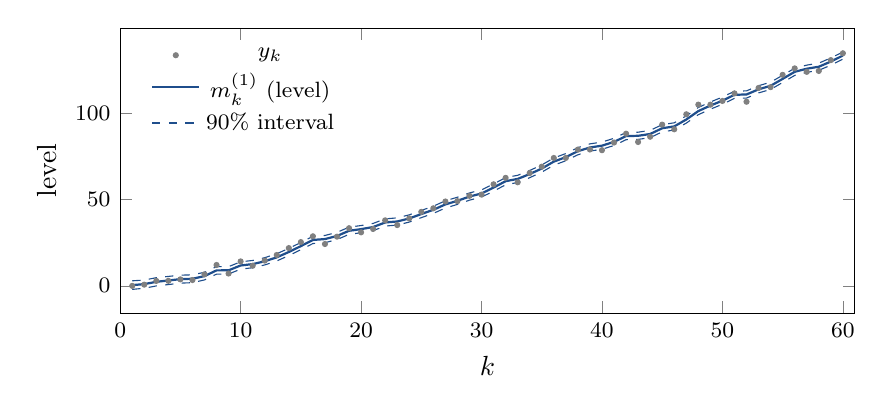
\begin{tikzpicture}
\begin{axis}[width=0.9\linewidth, height=5.2cm, xlabel={$k$}, ylabel={level}, xmin=0, xmax=61,
  legend pos=north west, legend style={font=\footnotesize, draw=none, fill=none}, tick label style={font=\footnotesize}]
\addplot[only marks, mark=*, mark size=0.9pt, gray] coordinates {(1,-0.020) (2,0.690) (3,2.840) (4,2.900) (5,3.750) (6,3.350) (7,6.650) (8,12.070) (9,7.120) (10,14.150) (11,11.640) (12,14.610) (13,17.850) (14,21.860) (15,25.320) (16,28.670) (17,24.190) (18,28.470) (19,33.350) (20,30.960) (21,32.930) (22,37.900) (23,35.170) (24,39.040) (25,42.810) (26,44.880) (27,48.810) (28,49.020) (29,52.080) (30,52.800) (31,58.760) (32,62.490) (33,59.920) (34,65.280) (35,68.970) (36,74.000) (37,74.020) (38,78.850) (39,78.900) (40,78.500) (41,82.930) (42,88.040) (43,83.240) (44,86.280) (45,93.290) (46,90.600) (47,99.290) (48,104.870) (49,104.840) (50,106.990) (51,111.360) (52,106.530) (53,114.510) (54,114.980) (55,122.100) (56,125.830) (57,123.830) (58,124.350) (59,130.620) (60,134.580)};
\addplot[thick, hwframe] coordinates {(1,0.421) (2,0.989) (3,2.333) (4,3.094) (5,3.877) (6,4.091) (7,5.641) (8,8.946) (9,8.979) (10,11.780) (11,12.581) (12,14.192) (13,16.491) (14,19.583) (15,22.996) (16,26.563) (17,27.063) (18,28.857) (19,31.861) (20,32.814) (21,34.032) (22,36.671) (23,37.250) (24,38.989) (25,41.547) (26,44.007) (27,47.125) (28,49.205) (29,51.665) (30,53.458) (31,56.873) (32,60.561) (33,61.886) (34,64.678) (35,67.877) (36,71.896) (37,74.473) (38,77.919) (39,80.073) (40,81.112) (41,83.310) (42,86.647) (43,86.826) (44,87.876) (45,91.195) (46,92.264) (47,96.263) (48,101.131) (49,104.322) (50,107.135) (51,110.562) (52,110.737) (53,113.719) (54,115.754) (55,119.770) (56,123.851) (57,125.645) (58,126.787) (59,129.799) (60,133.255)};
\addplot[dashed, hwframe] coordinates {(1,2.900) (2,3.359) (3,4.712) (4,5.453) (5,6.189) (6,6.350) (7,7.851) (8,11.115) (9,11.118) (10,13.898) (11,14.685) (12,16.287) (13,18.581) (14,21.670) (15,25.082) (16,28.648) (17,29.147) (18,30.942) (19,33.945) (20,34.899) (21,36.117) (22,38.756) (23,39.334) (24,41.073) (25,43.632) (26,46.091) (27,49.209) (28,51.290) (29,53.749) (30,55.543) (31,58.958) (32,62.645) (33,63.970) (34,66.763) (35,69.962) (36,73.980) (37,76.557) (38,80.003) (39,82.158) (40,83.197) (41,85.394) (42,88.732) (43,88.910) (44,89.960) (45,93.279) (46,94.348) (47,98.347) (48,103.215) (49,106.406) (50,109.220) (51,112.647) (52,112.821) (53,115.803) (54,117.838) (55,121.854) (56,125.936) (57,127.729) (58,128.871) (59,131.883) (60,135.339)};
\addplot[dashed, hwframe, forget plot] coordinates {(1,-2.058) (2,-1.382) (3,-0.047) (4,0.734) (5,1.564) (6,1.832) (7,3.431) (8,6.776) (9,6.839) (10,9.662) (11,10.477) (12,12.097) (13,14.402) (14,17.496) (15,20.911) (16,24.479) (17,24.978) (18,26.773) (19,29.776) (20,30.730) (21,31.948) (22,34.587) (23,35.166) (24,36.905) (25,39.463) (26,41.923) (27,45.040) (28,47.121) (29,49.581) (30,51.374) (31,54.789) (32,58.476) (33,59.801) (34,62.594) (35,65.793) (36,69.812) (37,72.388) (38,75.834) (39,77.989) (40,79.028) (41,81.226) (42,84.563) (43,84.742) (44,85.792) (45,89.110) (46,90.179) (47,94.178) (48,99.046) (49,102.238) (50,105.051) (51,108.478) (52,108.653) (53,111.635) (54,113.669) (55,117.686) (56,121.767) (57,123.561) (58,124.703) (59,127.714) (60,131.170)};
\legend{$y_k$, $m_k^{(1)}$ (level), $90\%$ interval}
\end{axis}
\end{tikzpicture}

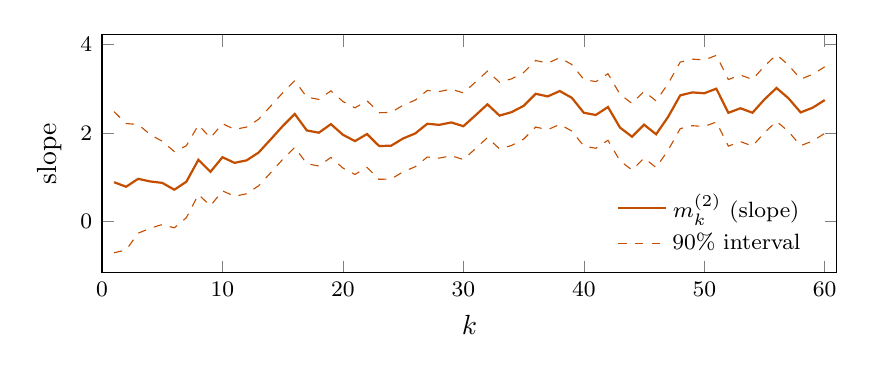
\begin{tikzpicture}
\begin{axis}[width=0.9\linewidth, height=4.6cm, xlabel={$k$}, ylabel={slope}, xmin=0, xmax=61,
  legend pos=south east, legend style={font=\footnotesize, draw=none, fill=none}, tick label style={font=\footnotesize}]
\addplot[thick, newterm] coordinates {(1,0.890) (2,0.788) (3,0.966) (4,0.907) (5,0.875) (6,0.721) (7,0.900) (8,1.395) (9,1.124) (10,1.452) (11,1.326) (12,1.381) (13,1.558) (14,1.853) (15,2.153) (16,2.426) (17,2.055) (18,2.004) (19,2.197) (20,1.957) (21,1.815) (22,1.974) (23,1.705) (24,1.711) (25,1.875) (26,1.987) (27,2.205) (28,2.181) (29,2.235) (30,2.150) (31,2.394) (32,2.643) (33,2.389) (34,2.467) (35,2.608) (36,2.880) (37,2.821) (38,2.942) (39,2.790) (40,2.453) (41,2.403) (42,2.583) (43,2.120) (44,1.914) (45,2.184) (46,1.969) (47,2.361) (48,2.844) (49,2.911) (50,2.892) (51,2.995) (52,2.452) (53,2.554) (54,2.454) (55,2.755) (56,3.011) (57,2.776) (58,2.461) (59,2.567) (60,2.739)};
\addplot[dashed, newterm] coordinates {(1,2.478) (2,2.211) (3,2.189) (4,1.962) (5,1.811) (6,1.579) (7,1.710) (8,2.177) (9,1.889) (10,2.209) (11,2.078) (12,2.131) (13,2.307) (14,2.602) (15,2.903) (16,3.175) (17,2.804) (18,2.754) (19,2.946) (20,2.707) (21,2.564) (22,2.723) (23,2.454) (24,2.461) (25,2.624) (26,2.737) (27,2.955) (28,2.931) (29,2.984) (30,2.899) (31,3.143) (32,3.392) (33,3.138) (34,3.216) (35,3.357) (36,3.629) (37,3.571) (38,3.691) (39,3.539) (40,3.202) (41,3.153) (42,3.333) (43,2.869) (44,2.663) (45,2.934) (46,2.719) (47,3.110) (48,3.593) (49,3.660) (50,3.642) (51,3.745) (52,3.201) (53,3.303) (54,3.203) (55,3.504) (56,3.760) (57,3.525) (58,3.210) (59,3.317) (60,3.488)};
\addplot[dashed, newterm, forget plot] coordinates {(1,-0.698) (2,-0.635) (3,-0.257) (4,-0.148) (5,-0.061) (6,-0.137) (7,0.090) (8,0.613) (9,0.358) (10,0.695) (11,0.573) (12,0.630) (13,0.808) (14,1.103) (15,1.404) (16,1.676) (17,1.305) (18,1.255) (19,1.448) (20,1.208) (21,1.065) (22,1.224) (23,0.955) (24,0.962) (25,1.125) (26,1.238) (27,1.456) (28,1.432) (29,1.486) (30,1.400) (31,1.644) (32,1.894) (33,1.640) (34,1.717) (35,1.859) (36,2.131) (37,2.072) (38,2.192) (39,2.041) (40,1.703) (41,1.654) (42,1.834) (43,1.371) (44,1.164) (45,1.435) (46,1.220) (47,1.611) (48,2.095) (49,2.162) (50,2.143) (51,2.246) (52,1.702) (53,1.804) (54,1.704) (55,2.006) (56,2.261) (57,2.027) (58,1.712) (59,1.818) (60,1.989)};
\legend{$m_k^{(2)}$ (slope), $90\%$ interval}
\end{axis}
\end{tikzpicture}
\end{center}

\setcounter{enumi}{5}
\item Each forecast step applies only the prediction step, with no update, so the uncertainty keeps growing. With $H = (1\ \ 0)$, $H\mt_k = \mt_k^{(1)}$ and $S_k = \Pt_k^{(1,1)} + R$:
\begin{center}
\begin{tabular}{ccc}
\toprule
step & mean $H\mt_k$ & $90\%$ interval\\
\midrule
$T+1$ & $135.99$ & $[131.74,\ 140.25]$\\
$T+2$ & $138.73$ & $[134.02,\ 143.45]$\\
$T+3$ & $141.47$ & $[136.20,\ 146.74]$\\
$T+4$ & $144.21$ & $[138.29,\ 150.13]$\\
$T+5$ & $146.95$ & $[140.30,\ 153.60]$\\
$T+6$ & $149.69$ & $[142.24,\ 157.13]$\\
$T+7$ & $152.42$ & $[144.12,\ 160.73]$\\
$T+8$ & $155.16$ & $[145.94,\ 164.39]$\\
$T+9$ & $157.90$ & $[147.71,\ 168.09]$\\
$T+10$ & $160.64$ & $[149.43,\ 171.85]$\\
\bottomrule
\end{tabular}
\end{center}
The mean grows linearly, by about the filtered slope $2.74$ per step, and the interval widens: the slope uncertainty enters the level quadratically through $A$.

\item The noise ratio $Q/R$ controls how much the filter trusts each new measurement. At the end of the series:
\begin{center}
\begin{tabular}{cccc}
\toprule
$R$ & $K_T^{(1)}$ (level gain) & $K_T^{(2)}$ (slope gain) & $\sqrt{P_T^{(1,1)}}$\\
\midrule
$1$ & $0.553$ & $0.134$ & $0.74$\\
$4$ & $0.401$ & $0.077$ & $1.27$\\
$16$ & $0.289$ & $0.042$ & $2.15$\\
\bottomrule
\end{tabular}
\end{center}
A small $R$ says the measurements are precise: the gain is large and the level follows the data closely. A large $R$ gives a smaller gain and a smoother estimate, which reacts more slowly to real changes, and a wider interval for the level.
\end{enumerate}
\end{homework}

%=====================================================
\section*{References}
\begin{itemize}
\item S\"arkk\"a, S. (2013). \emph{Bayesian Filtering and Smoothing}. Cambridge University Press. Chapter 4: probabilistic state-space models, the Bayesian filtering equations and the Kalman filter, with the same notation as these notes.
\item Kalman, R.~E. (1960). A new approach to linear filtering and prediction problems. \emph{Journal of Basic Engineering}, 82(1), 35--45. The original paper.
\item Bishop, C.~M. (2006). \emph{Pattern Recognition and Machine Learning}. Springer. Section 13.3: linear dynamical systems.
\end{itemize}

\end{document}
